% !Mode:: "TeX:UTF-8"
% !TEX program  = xelatex

\documentclass{cumcmthesis}
%\documentclass[withoutpreface,bwprint]{cumcmthesis} %去掉封面与编号页

\usepackage{url}
\title{基于非稳态导热的高温作业专用服装设计}
\tihao{A}
\baominghao{ }
\schoolname{华中科技大学}
\membera{陆敏铖}
\memberb{汤若水}
\memberc{顾轩}
\supervisor{}
\yearinput{2019}
\monthinput{08}
\dayinput{18}

\begin{document}

 \maketitle
 \begin{abstract}
    本文通过传热学知识,结合了克兰克-尼科尔森方法,追赶法与相似对角化法等一系列方法,加上一些数值求解的技巧,构建了一套预测在高温环境下防护服内部的温度变化趋势的
    体系,并用这套体系预测了皮肤表面温度在特定条件下的变化,与实验数据符合较好.之后,继续使用这一套模型预测高温防护服在不同情况下的温度变化,来辅助防护服的设计,简化
    高温防护服的设计流程

    \keywords{克兰克-尼科尔森方法\quad  曲线拟合\quad   非线性优化模型\quad  受力分析}
\end{abstract}

%目录
\tableofcontents
\newpage
\section{问题重述}

    \subsection{问题背景}
        服装作为人与环境之间的中间体,它的功能,逐渐由最原始的遮体避寒,发展出
        许多不同的功能特性,以此来保证人类能适应现代快速发展的社会,能够从事相应的,
        有不同要求的生产活动。现代材料学、工程学、以及基础科学的快速发展,使得服装
        有了更为复杂多样,且更为有效的功能。因而不同环境下的服装性能被愈加重视。

        现代工业生产中,不可避免会出现有与普通环境完全不同的工作环境,包括高温、
        低温、缺氧、无菌、辐射等,其中高温环境作为生产与作业中最常出现的一种情况,
        高温作业专用服装的设计被高度重视,国内外在该方面拥有广泛而深入的研究。

            在本文中,将建立高温作业专用服装的数学模型,分析在不同温度、不同时间、不同
        材质情况下的高温作业专用服的隔热情况,并由此根据环境对皮肤温度进
        行合理评估,进而通过温度要求对服装厚度和材料选取实现最优设计。

    \subsection{问题重述}

        高温环境下工作时人们需要穿着专用服装以避免灼伤。专用服装通常由三
        层织物材料构成,I层与外界环境接触,III层与皮肤之间还存在空隙,空隙记为IV层。

        为设计专用服装,将体内温度控制在37ºC的假人放置在实验室的高温环境中,测量
        假人皮肤外侧的温度。为了降低研发成本、缩短研发周期,请你们利用数学模型来确
        定假人皮肤外侧的温度变化情况,并解决以下问题:

        (1) 专用服装材料的某些参数值由附件1给出,对环境温度为75ºC、II层厚度为6 mm、
        IV层厚度为5 mm、工作时间为90分钟的情形开展实验,测量得到假人皮肤外侧的
        温度(见附件2)。建立数学模型,计算温度分布,并生成温度分布的Excel文件
        (文件名为problem1.xlsx)。

        (2) 当环境温度为65ºC、IV层的厚度为5.5 mm时,确定II层的最优厚度,确保工作60
        分钟时,假人皮肤外侧温度不超过47ºC,且超过44ºC的时间不超过5分钟。
    
        (3) 当环境温度为80 时,确定II层和IV层的最优厚度,确保工作30分钟时,假人皮肤
        外侧温度不超过47ºC,且超过44ºC的时间不超过5分钟。
\section{问题分析}
    \subsection{问题一的分析}

        问题一要求建立温度在时间和空间上的分布函数,在各阻热层各向同性的假设下,仅需
        考虑一维情况下的温度分布。考虑热量传输过程,该过程有75℃和37℃两个恒温源
        在75℃边界上主要考虑热对流,在中间四层介质中热量主要以热传导方式进行传递,皮肤
        表面和37℃恒温源之间仍然主要考虑热对流形式。
        
        因此,问题一需要建立基于热传导的温度分布模型,由傅里叶定律和能量守恒定律推导出四层介质的热传导方程。根据
        初始时刻的温度分布都为37℃建立初始条件,与热传导过程温度场的连续性建立各层介质之间的
        衔接条件,和高温恒温热源以及低温恒温热源处的热对流方程(传热系数未知)来确定方程
        的边界条件。
        
        由于向前差分方程在\(\Delta x\)过小,\(\Delta t\)过大时,会出现振荡情况,因此考虑将微分方程转化为
        精度较高的克兰克-尼科尔森差分方程\cite{wiki}。
        
        由于求出的系数矩阵\(\bf{R_p},\bf{R_n}\)
        都是三对角矩阵,可以快速求逆,再加上对不动点的利用,可以快速求出皮肤表面温度关于时间的变化曲线,
        该曲线与热对流方程的传热系数有关,利用附件2测量所得假人皮肤外侧温度,通过最小二乘法
        求出皮肤表面温度关于时间函数与实际情况最接近时的传热系数,最后由求得的传热系数
        求出温度在时间和空间上的分布并生成表格。

    \subsection{问题二的分析}

        问题一建立了温度在时间和空间上的分布函数,由高温恒温热源、低温恒温热
        源、传热系数、各介质相关性质可以求出任意时间和空间上的温度值;

        问题二是求解 II 层介质最优厚度的一个最优化问题,从服装成本最低与穿着
        舒适度最高两方面考虑需求取II层介质厚度的最小值,其约束条件为假人皮肤外侧温
        度60分钟时不超过47ºC,55分钟时不超过44℃。因此我们使用二分查找法,对
        II 层介质的所有可能厚度进行遍历,最终求出满足约束条件的最小厚度。


    \subsection{问题三的分析}

        问题三是求解 II,IV 两层的最优厚度的一个多目标的优化问题。
        
        类似于问题二,
        需要求取满足约束条件情况下的II,IV 两层的厚度使服装成本最低和穿着舒适度最高。
        该问题约束条件为假人皮肤外侧温度30分钟时不超过47ºC,25分钟时不超过44℃.考虑
        对对II 介质与 IV 介质厚度进行双重循环遍历,寻找到满足约束条件的II、IV两层厚度
        范围,最终根据服装成本最低和穿着舒适度最高的目标确定 II,IV 两层的最优厚度。
\section{模型假设}

\begin{itemize}
\item 假设各层介质都是各向同性;
\item 假设恒温源处的热辐射和热传导可以忽略,仅考虑热对流;
\item 假设每层介质的热传导率在各个方向相同;
\item 假设衣服形状规则,各层介质可被视为平行材料不发生扭曲;
\item 假设温度测量准确,皮肤表面各处温度相同;
\item 假设长时间的实验过程衣服材料的导热率等参数保持不变;
\item 热对流仅仅发生在边界一小段距离内.
\end{itemize}


\section{符号说明}
    \begin{center}
    \begin{tabular}{cc}
    \hline
    \makebox[0.3\textwidth][c]{符号}	&  \makebox[0.4\textwidth][c]{意义} \\ \hline
    x               & 位置  \\ \hline
    k               & 热传导率  \\ \hline
    \(\rho\)        & 密度  \\ \hline
    c               & 比热容  \\ \hline
    t               & 时间      \\ \hline
    u(x,t)          & 温度  \\ \hline
    q               & 热流量  \\ \hline
    h               & 固体表面的平均表面换热系数  \\ \hline
    \(\bf{a}\)      & 加粗小写字母表示向量  \\ \hline
    \(\bf{A}\)      & 加粗大写字母表示矩阵  \\ \hline
    \(\bf{A}^n\)    & 矩阵的n次幂  \\ \hline


    \end{tabular}
    \end{center}


\section{模型建立与求解}

    \subsection{问题一:确定温度分布情况} 
        \paragraph{问题的分析}

            问题一主要求解皮肤表面的温度变化曲线,通过观察测量数据可以发现,在90分钟的时候,防护服内已经达到了热平衡.

            由此,我们可以确定两侧换热系数的关系,并且在建立差分方程后,根据总方差最小的原则,取到一组合适的换热系数,并且以此预测
            皮肤表面的温度变化曲线.

        \paragraph{模型的建立}

            给定区间 \([x_{i-1},x_i]\),每个区间上都有热力学参数:\(k_i,\rho_i,c_i\),三者
            分别为该区间上热传导率、密度和比热容,其中\(i=0,1,2,3,4\)。

            从而可以得到热传导方程\cite{book}:
            \[k\frac{\partial^2 u}{\partial x^2} = \frac{\partial u}{\partial t}\rho c |_{x_{i-1}<x<x_{i}}\] 
            由于该高温服装由多层不同材质的物料组成,所以在不同介质交换处,由
            \(\frac{\partial{q}}{\partial{x}} = \frac{\partial{u}}{\partial{t}} \rho c \)
            可得:
            \[ 
                \lim_{\delta \to 0^+} 
                k_{i+1 }\frac{\partial{u(x_i+\delta)}}{\partial{x}} 
                -
                \int_{x_i}^{x_i+\delta}\frac{\partial{u}}{\partial{t}} \rho_{i+1} c_{i+1} dx 
                = 
                \lim_{\delta \to 0^+} 
                k_{i} \frac{\partial{u(x_i-\delta)}}{\partial{x}}
                - 
                \int_{x_i}^{x_i-\delta}\frac{\partial{u}}{\partial{t}} \rho_i c_i dx
                =
                q(x_i)
            \]

            此外,在这个高温工作服的两端,都有空气存在。空气层与其他固体介质层有
            着巨大的差异。空气层具有流体性质,所以在两端,还要考虑对流换热的存在。
            对流换热是流体的导热和热对流两种基本方式共同作用的结果。
            在左端,由牛顿冷却公式\(q = h\Delta u\)
            因而有:
            \[
                \lim_{\delta \to 0^+} 
                k\frac{\partial{u(\delta)}}{\partial{x}} 
                - 
                h[u(0) - u_w]
                -
                \int_{0}^{\delta}\frac{\partial{u}}{\partial{t}} \rho c dx 
                = 0
            \]
            右端在高温工作服表面也是类似的空气流动,同样是这样的原理和公式。

            在单一介质内部,我们采用克兰克-尼科尔森差分法(C-N方法)做差分,将每一部分看做一个小单元,分析它热量的变化
            \[(q_{i+1} - q_{i+1})\Delta t = \rho c \Delta x\]

            \begin{figure}[ht] 
                \centering 
                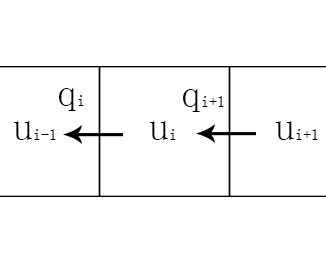
\includegraphics[scale=0.9]{../figure/diff.png} 
                \caption{区块模拟图}\label{diff}    
            \end{figure}
            可以得到:
            \[
                \frac{1}{2}
                \left(
                    \frac{u_{i+1}^{n+1} + u_{i-1}^{n+1} - 2u_{i}^{n+1} }{\Delta x^2}
                    +
                    \frac{u_{i+1}^{n} + u_{i-1}^{n} - 2u_{i}^{n} }{\Delta x^2}
                \right)
                k
                =
                \frac{ u_{i}^{n+1} - u_{i}^{n} }{\Delta t} \rho c
            \]
            我们可以记:
            \( r = \frac{k \Delta t}{ 2 \rho c \Delta x^2 } \)
            整理上式可以得到:
            \[
                -ru_{i+1}^{n+1} + (1+2r)u_{i}^{n+1} + -ru_{i-1}^{n+1}
                =
                ru_{i+1}^{n} + (1-2r)u_{i}^{n} + ru_{i-1}^{n}
            \]
            这就是单一介质内部的温度变化与分布规律。

            由于实际上的高温工作服,由多层复合材质组成,层与层之间
            存在着不同的导热系数,所以单一介质的传热规律在不同层之间不能很
            好符合。在介质交界处我们需要另外考虑。

            假设小区块分成两半,每一半介质不同,记前一种介质的热传导率为\(k_p\),后一种介质的热传导率为\(k_n\),
            \(\rho c\)是前后两种介质单位体积热容的平均值,有:
            \[
                \frac{1}{2}
                \left[
                    \frac{k_n u_{i+1}^{n+1} + k_p u_{i-1}^{n+1} - (k_p+k_n)u_{i}^{n+1}) }{\Delta x^2}
                    +
                    \frac{k_n u_{i+1}^{n} + k_p u_{i-1}^{n} - (k_p+k_n)u_{i}^{n} }{\Delta x^2}
                \right]
                =
                \frac{ u_{i}^{n+1} - u_{i}^{n} }{\Delta t} \rho c
            \]
            在两端处,以左端为例:
            \[
                \frac{1}{2}
                \left[
                    k\frac{ u_{2}^{n+1}  - u_{1}^{n+1} }{\Delta x}
                    -
                    h_l(u_{1}^{n+1} - u_w)
                    +
                    k\frac{ u_{2}^{n}  - u_{1}^{n} }{\Delta x}
                    -
                    h_l(u_{1}^{n} - u_w)
                \right]
                =
                \frac{ u_{i}^{n+1} - u_{i}^{n} }{\Delta t} \rho c \frac{\Delta x}{2}
            \]
            根据这样多重线性映射的关系,得到递推式:
            \[\bf{R_n}\bf{u}^{n+1} = \bf{R_p}\bf{u}^{n} + \bf{q}\]
            记:
            \[\bf{A} = \bf{R}_n^{-1}\bf{R}_p\]
            \[\bf{b} = \bf{R}_n^{-1}\bf{q}\]
            有递推关系式
            \[\bf{u}^{n+1} = \bf{A}\bf{u}^{n} + \bf{b}\]
            记这个映射有不动点:
            \[\bf{u}_s = \bf{A}\bf{u}_s + \bf{b}\]
            则有:
            \[ \bf{u}^{n+1} - \bf{u}_s = \bf{A} (\bf{u}^n - \bf{u}_s) \]
            即:
            \[\bf{u}^{n} = \bf{A}^n (\bf{u}^0 - \bf{u}_s) + \bf{u}_s\]
            显然的:
            \[\bf{u}_s = (\bf{I} - \bf{A})^{-1}\bf{b}\]
            这样就可以快速的求解任意时刻的温度分布:
            \[\bf{u}|_{t = t_0} = \bf{A}^{\frac{t_0}{\Delta t}} (\bf{u}^0 - \bf{u}_s) + \bf{u}_s\]

        \paragraph{模型的求解}

            记\(h_l,h_r\)分别为左右两边的换热系数,\(u_l,u_r\)分别为左右两边的温度,\(u_{wl},u_{wr}\)分别为左右两边的环境温度
            根据稳态的热平衡,我们可以列出如下关系式:
            \[\sum_{i=1}^4 \frac{L_i}{k_i} + \frac{1}{h_l} + \frac{1}{h_r} = \frac{u_{wr}-u_{wl}}{q}\]
            又由热平衡:\( h_r(u_l-u_{wl}) = q\)
            不难得出\(h_r,h_l\)的关系:
            \[h_l = \frac{\alpha h_r}{1+\beta hr}\]
            其中参数\(\alpha = 2.4296 ,\beta = 0.2821\)
            不难发现\(h_r\)大致在80~120之间,我们在这个区间上二分查找一个\(h_r\),使得计算数据与原始数据的总标准差:
            \[S = \sqrt{\frac{\sum_{i=1}^{N}(u_i-\hat{u_i})^2}{N}}\]
            取得最小值
            计算可得\(h_r\)大致为:100.63,\(h_l\)大致为8.319,相对应的\(S = 0.052\)
            \(S-h_r\)的关系见下图:
            \begin{figure}[ht] 
                \centering 
                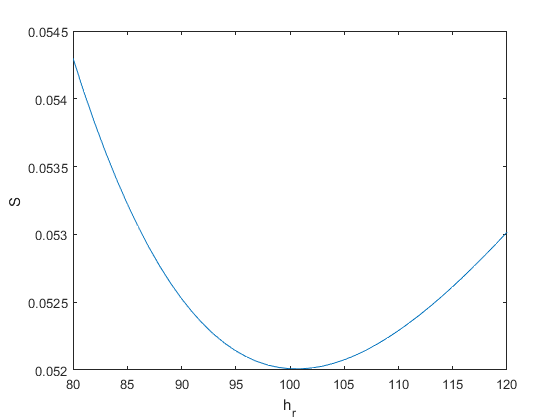
\includegraphics[scale=0.9]{../figure/ques1Optimization.png} 
                \caption{\(S-h_r\)的关系}\label{optimization}    
            \end{figure}
        \paragraph{结果的分析和检验}

            将实际测量的\textbf{皮肤表面温度变化曲线}与理论得到的\textbf{皮肤表面温度变化曲线}绘制在一张图上
            \begin{figure}[ht] 
                \centering 
                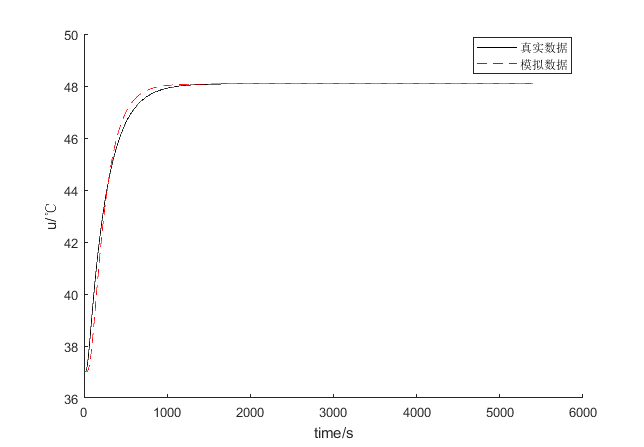
\includegraphics[scale=0.9]{../figure/ques1result.png} 
                \caption{实际数据与计算结果的对比}\label{cou}    
            \end{figure}


    \subsection{问题二:确定II层介质最优厚度} 
        \paragraph{问题的分析} 
        
            在问题一中求出最符合实验结果的传热系数h,问题2需要求解满足约束条件下的II层介质最优厚度,该问题为单一变量的优化问题,
            目标为服装成本最低与穿着舒适度最高。
            易知当材料厚度最小时成本最低且舒适度最高。因此问题2为在满足条件:
                \[
                    \left\{
                        \begin{aligned}
                            u|_{x=0mm,t=3300s}&<44^{\circ}C\\
                            u|_{x=0mm,t=3600s}&<47^{\circ}C
                        \end{aligned}
                    \right.     
                \]
            情况下,求取II层介质厚度\(L_2\)的最小值\(\min{L_2}\)。
        \paragraph{模型的求解}
            采用二分查找的方法,确定II层介质的最小厚度,在II层介质的允许厚度中进行枚举,得出不同介质厚度相对应的55分钟和60分钟时的温度\(u_{3300}\),通过(****约束条件)
            找到II层介质的临界值,该临界值即为所求目标:\(\min{\L_2}\)。

            通过matlab所得II层厚度\(L_2\)与55分钟的皮肤表面温度\(u_{3300}\)的关系如图:

            \begin{figure}[ht] 
                \centering 
                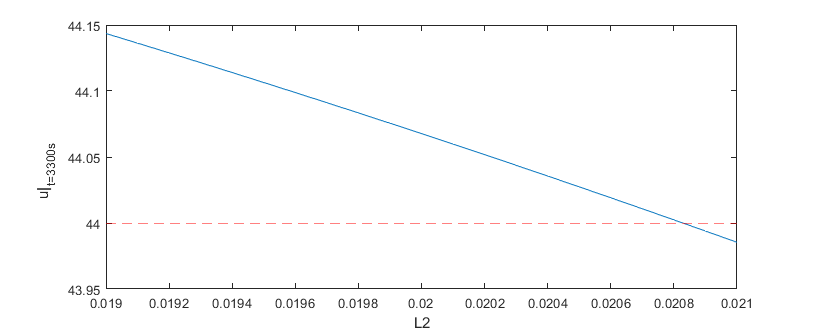
\includegraphics[scale=0.7]{../figure/ques2result.png} 
                \caption{\(L_2 - u_{3300}\)}\label{fig:one}    
            \end{figure}

            由图可知,\(L_2 = 20.9mm\)时,\(u_{3300}\)恰好小于44℃一点,而60分钟的皮肤表面温度\(u_{3600}\)达不到47℃,由此可得满足约束条件的II层厚度的临界值为20.9mm,
            由上面分析可知,该临界厚度为II层介质最优厚度。所以最终得到\(L2\)的最优厚度为20.9mm


     \subsection{问题三:确定II、IV层介质最优厚度} 
        \paragraph{问题的分析}
            与问题二类似,问题三仍需要求解满足约束条件下的II、IV层介质最优厚度,该问题变为双变量的优化问题,目标为服装成本最低与穿着舒适度最高。因此可以考虑求出
            满足条件:
            \[
                \left\{
                    \begin{aligned}
                        u|_{x=0mm,t=1500s}&<44^{\circ}C\\
                        u|_{x=0mm,t=1800s}&<47^{\circ}C
                    \end{aligned}
                \right.     
            \]
            的II、IV层介质厚度的组合,在所有组合中寻找到使服装成本最低、穿着舒适度最高的II、IV层介质厚度。
        \paragraph{模型的求解} 

        

            对II 介质与 IV 介质厚度进行双重循环遍历,寻找到满足约束条件的II、IV两层厚度范围,得出不同的II、IV厚度与1500秒时皮肤表面温度关系如图:
            \begin{figure}[ht] 
                \centering 
                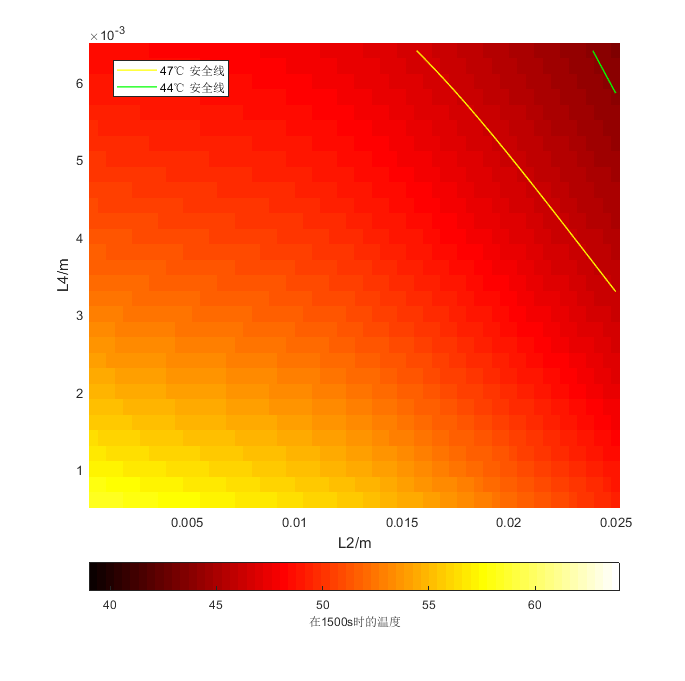
\includegraphics[scale=0.9]{../figure/ques3HeatMapByL2L4.png} 
                \caption{1500s后皮肤表面温度与\(L_2,L_4\)的关系}\label{diff}    
            \end{figure}

            在图[5]上做出使得1500s时皮肤表面温度为44℃的\(L_2,L_4\)曲线(图中绿线),与1800s时皮肤表面温度为47℃的曲线(图中黄线)
            由约束条件可知在该线右上部分为满足条件的II、IV厚度范围。通过取步长为0.1mm,
            得到一系列临近分布在图中绿线右上的点,显然这些点是恰好使得温度在1500s的时候不超过44℃,并且厚度尽可能小的:

            (24.04,6.4)\quad(24.24 6.3)\quad(24.44 6.2)\quad(24.54 6.1)\quad(24.84 6.0)
        
            由上述列举的点可以发现,\(L_2 = 24.04mm,L_4 = 6.4mm\)时,使得高温作业专用服装的厚度达到最小值,此时服装成本最低且此时穿着舒适度最高。因此可以得到:
            满足假人皮肤外侧温度30分钟时不超过47ºC,25分钟时不超过44℃的II层介质最优厚度为24.04mm,IV层介质最优厚度为6.4mm。
    
\section{模型的评价和推广}
    \subsection{模型优点} 
        \begin{itemize}
            \item 利用Crank-Nicolson 差分格式对连续的模型进行离散化处理进行数值求解,对前后差分取平均值,能够获得误差更小的数值解;
            \item 在求解一定时刻的温度分布\(\bf{u}_t\)时,采用寻找不动点\(\bf{u}_s\)后直接做矩阵乘法的方法,极大提高了运算速度,可以较快求解;
            \item 第三类边界条件由牛顿冷却方程得出,并合理考虑热传导的影响,使模型的建立更加接近实际情况;
            \item 由物理传热规律求出两个传热系数之间的关系,进而减少变量对单一变量进行研究,结果误差更小;
        \end{itemize}
    \subsection{模型缺点}
        \begin{itemize}
            \item 在进行克兰克-尼科尔森差分法时,需要对数据进行离散化处理,会导致结果不精确;
            \item 边界的对流情况其实十分复杂,这个模型仅仅考虑了一小段物质建立对流换热方程
        \end{itemize}
    \subsection{模型推广}
        在本文中,我们建立了高温作业专用服装的数学模型,分析在不同温度、不同时间、不同
        材质情况下的高温作业专用服的隔热情况,进而通过温度要求对服装厚度和材料选取实现
        最优设计。不过我们目前设计的模型是在一维层面的,可以将其推广到二维,三维环境,
        以更符合现实情况。此外,我们建立的是一个传热的基本模型,所以可以将这个模型推广
        到其他热学问题领域。
\section{参考文献}


%参考文献
\begin{thebibliography}{9}%宽度9
 \bibitem{wiki} 克兰克——尼克尔森方法 [G/OL]. 维基百科, 2016.7.11[2019.8.15].
 \bibitem{book} [TK124] 陈维汉.工程传热学[M].武汉:华中科技大学出版社,2011.
\end{thebibliography}

\newpage
%附录
\begin{appendices}
\section{C-N方法的matlab代码}
\begin{lstlisting}[language=matlab]
    function u_alltime = getUt(hl,hr)
    u_0 = 37;
    u_end = 75;
    %hl = 8.318143355830285;
    %hr = 1.002000000000000e+02;
    total_time = 5400;
    del_x = 1e-4;
    del_t = 0.01;
    L1 = 0.6/1000;
    L2 = 6/1000;
    L3 = 3.6/1000;
    L4 = 5/1000;
    x43 = L4;
    
    x32 = L4+L3;
    
    x21 = L4+L3+L2;
    
    x0 = 0;
    xend = L4+L3+L2+L1;
    xp = [x0,x43,x32,x21,xend];
    %t = 0:del_t:300;
    N = round(xend/del_x+1);
    Rp = zeros(N,N);
    Rn = zeros(N,N);
    delta = zeros(N,1);
    r4 = del_t*2.361075976051944e-05/(2*del_x^2);
    r3 = del_t*3.441935316092042e-07/(2*del_x^2);
    r2 = del_t*2.043973041652856e-07/(2*del_x^2);
    r1 = del_t*1.984991527475188e-07/(2*del_x^2);
    rs = [r1,r2,r3,r4];
    
    k4 = 0.028;
    k3 = 0.045;
    k2 = 0.37;
    k1 = 0.082;
    k = [k4,k3,k2,k1];
    
    rho4 = 1.18;
    rho3 = 74.2;
    rho2 = 862;
    rho1 = 300;
    rho = [rho4,rho3,rho2,rho1];
    
    c4 = 1055;
    c3 = 1726;
    c2 = 2100;
    c1 = 1377;
    c = [c4,c3,c2,c1];
    
    
    %R_n * u_n+1 = R_p * u_n + b
    
    
    %Rp(1,1) = k4/del_x + hl;
    %Rp(1,2) = -k4/(del_x);
    
    %Rn(1,1) = -hl-k4/del_x;
    %Rn(1,2) = -k4/(del_x);
    d_edge = 0.5*del_x;
    Rp(1,1) = - k4/(2*del_x*d_edge) - hl/(2*d_edge) + rho4*c4/del_t;
    Rp(1,2) = k4/(2*del_x*d_edge);
    
    Rn(1,1) = k4/(2*del_x*d_edge) + hl/(2*d_edge) +  rho4*c4/del_t;
    Rn(1,2) = -k4/(2*del_x*d_edge);
    
    delta(1) = hl*u_0/d_edge;
    
    
    
    for region = 1:4
        a = round(2 + xp(region)/del_x);
        b = round(xp(region+1)/del_x);
        r = rs(region);
        for index = a:b
    
            Rp(index,index-1) = r;   
            Rp(index,index) = 1-2*r;
            Rp(index,index+1) = r;
        
            Rn(index,index-1) = -r;
            Rn(index,index) = 1 + 2*r;
            Rn(index,index+1) = -r ;
        end
        index = index + 1;
        % (u_{i+1} - u_{i})*k_{next} = (u_{i} - u_{i-1})*k_{pre}
        
        if region == 4
            Rp(index,index-1) = k1/(2*del_x*d_edge);
            Rp(index,index) = - k1/(2*del_x*d_edge) - hr/(2*d_edge) + rho1*c1/del_t;
            Rn(index,index) = rho1*c1/del_t + k1/(2*del_x*d_edge) + hr/(2*d_edge);
            Rn(index,index-1) = -k1/(2*del_x*d_edge);
            delta(N) = hr*u_end/(d_edge);
        else
            kn = k(region+1);
            kp = k(region);
    
            rhocm = 0.5*c(region)*rho(region)+0.5*c(region+1)*rho(region+1);
            
            rn = del_t*kn/(rhocm*2*del_x^2);
            rp = del_t*kp/(rhocm*2*del_x^2);
            Rp(index,index-1) = rp;   
            Rp(index,index) = 1-rn-rp;
            Rp(index,index+1) = rn;
    
            Rn(index,index-1) = -rp;
            Rn(index,index) = 1+rn+rp;
            Rn(index,index+1) = -rn;
        end
    end
    
    
    
        A = Rn\Rp;
        b = Rn\delta;
        u_s = (eye(N)-A)\b;
        u_t = ones(N,1)*37.0;
        u_del = u_t - u_s;
        A_dt = A^100;
        
        u_alltime = zeros(total_time+1,1);
        i = 1;
        for time = 0:1:total_time
            u_alltime(i) = u_t(1);
            u_del = A_dt*u_del;
            u_t = u_del + u_s;
            i = i +1;
        end
    end
\end{lstlisting}

\end{appendices}

\end{document} 